\documentclass[a4paper,12pt]{article}

% ---------------- Encoding & Language ----------------
\usepackage[utf8]{inputenc}
\usepackage[T5]{fontenc} % better for Vietnamese diacritics
\usepackage[english,vietnamese]{babel}

% ---------------- Packages ----------------
\usepackage{amsmath,amssymb}
\usepackage{array}
\usepackage{textcomp}
\usepackage{xcolor}
\usepackage{graphicx}
\usepackage{geometry}
\usepackage{float}
\usepackage{mdframed}
\usepackage{nopageno}
\usepackage{fancyhdr}
\usepackage{ulem}
\usepackage{tcolorbox}
\usepackage{tocloft}
\usepackage{hyperref}
\usepackage{subcaption}
\usepackage{listings}
\usepackage{longtable}
\usepackage{booktabs}
\usepackage{tabularx}
\usepackage{adjustbox}

% ---------------- Page setup ----------------
\geometry{a4paper, margin=0.75in}
\setlength{\parindent}{0pt} % remove paragraph indentation so lines start flush left

\mdfdefinestyle{MyFrame}{%
    linecolor=blue,
    outerlinewidth=2pt,
    roundcorner=0pt,
    innertopmargin=10pt,
    innerbottommargin=10pt,
    innerrightmargin=10pt,
    innerleftmargin=10pt,
    backgroundcolor=white
}

% ---------------- Colors for listings ----------------
\definecolor{comment}{RGB}{0,128,0}   % green for comments
\definecolor{kwpink}{RGB}{255,20,147} % pink for keywords
\definecolor{numblue}{RGB}{0,0,200}   % blue for numeric literals
\definecolor{string}{RGB}{163,21,21}  % string color (dark red)
\definecolor{framegray}{RGB}{200,200,200}

% ---------------- Listing configuration ----------------
% ---------------- Listing configuration ----------------
\lstset{
    language=C,                       % use C syntax highlighting
    basicstyle=\ttfamily\small,
    keywordstyle=\color{kwpink}\bfseries, % pink for keywords
    commentstyle=\color{comment}\itshape, % green comments
    stringstyle=\color{string},        % dark red strings
    numbers=left,
    numberstyle=\tiny\color{gray},
    stepnumber=1,
    numbersep=6pt,
    backgroundcolor=\color{white},
    frame=single,
    rulecolor=\color{framegray},
    breaklines=true,
    tabsize=4,
    showspaces=false,
    showstringspaces=false,
    alsoletter={_},
    morekeywords={if,else,while,for,switch,case,return}, % only control-flow pink
    deletekeywords={HAL_Delay}, % make sure HAL_Delay is not colored as keyword
    literate=%
     *{0}{{{\color{numblue}0}}}1
      {1}{{{\color{numblue}1}}}1
      {2}{{{\color{numblue}2}}}1
      {3}{{{\color{numblue}3}}}1
      {4}{{{\color{numblue}4}}}1
      {5}{{{\color{numblue}5}}}1
      {6}{{{\color{numblue}6}}}1
      {7}{{{\color{numblue}7}}}1
      {8}{{{\color{numblue}8}}}1
      {9}{{{\color{numblue}9}}}1
      {.}{{{\color{numblue}.}}}1
}

% ---------------- Header / Footer ----------------
\pagestyle{fancy}
\fancyhf{}
\fancyhead[L]{\small Ho Chi Minh City University of Technology \\ Faculty of Computer Science and Engineering}
\fancyhead[R]{
\includegraphics[height=20pt]{bk_logo.png}}
\fancyfoot[C]{\thepage}
\renewcommand{\headrulewidth}{1.5pt}
\renewcommand{\footrulewidth}{1.5pt}

% ---------------- Document ----------------
\begin{document}
\selectlanguage{vietnamese}

\begin{mdframed}[style=MyFrame]
\thispagestyle{empty}
\begin{center}
    \vspace*{0.5cm}
    {\large \textbf{TRƯỜNG ĐẠI HỌC BÁCH KHOA – TP. HỒ CHÍ MINH}}\\[0.2cm]
    {\large \textbf{KHOA KHOA HỌC VÀ KỸ THUẬT MÁY TÍNH}}\\[0.5cm]
    \textbf{*******************}\\[1cm]

    
\includegraphics[width=0.3\textwidth]{bk_logo.png}\\[2cm]

    {\LARGE \textbf{Lab 3 - Buttons - Switchs}}\\[0.5cm]
    {\LARGE \textcolor{blue}{Microcontroller - Microprocessor (Lab)}}\\[0.5cm]
    {\LARGE \textbf{COURSE ID: CO3010 - HK251}}\\[0.5cm]
    \textbf{\large Name: Trương Gia Hy   -   Student ID: 2352458}\\[0.5cm]
    \textbf{\large Supervising Lecturer: Dr. VÕ TUẤN BÌNH}\\[8.5cm]

    {\large TP. Hồ Chí Minh – 2024}
\end{center}
\end{mdframed}

\newpage
\section{Exercises and Report}
\subsection{Specifications}
\begin{itemize}
	\item[] You are required to build an application of a traffic light in a cross road which includes
	some features as described below:
	\begin{itemize}
		\item[\textbullet] The application has 12 LEDs including 4 red LEDs, 4 amber LEDs, 4 green LEDs.
		\item[\textbullet] The application has 4 seven segment LEDs to display time with 2 for each road. The
		2 seven segment LEDs will show time for each color LED corresponding to each
		road.
		\item[\textbullet] The application has three buttons which are used
		\item[] \hspace{0.5cm} - to select modes,
		\item[] \hspace{0.5cm} - to modify the time for each color led on the fly,
		\item[] \hspace{0.5cm} - to set the chosen value.
	\end{itemize}
	\item[\textbullet] The application has at least 4 modes which is controlled by the first button. Mode 1 is a normal mode, while modes 2 3 4 are modification modes. You can press the
	first button to change the mode. Modes will change from 1 to 4 and back to 1 again.
	\begin{itemize}
		\item[] \textbf{Mode 1 - Normal mode:}
		\begin{itemize}
			\item[] - The traffic light application is running normally.
		\end{itemize}
		\item[] \textbf{Mode 2 - Modify time duration for the red LEDs:} This mode allows you to change the time duration of the red LED in the main road. The expected behaviours of this
		mode include:
		\begin{itemize}
			\item[] - All single red LEDs blink at 2 Hz.
			\item[] - Two seven-segment LEDs display the time value.
			\item[] - The other two seven-segment LEDs display the mode.
			\item[] - The second button increases the time duration value for the red LEDs.
			\item[] - The time duration value ranges from 1 to 99.
			\item[] - The third button sets the value.
		\end{itemize}
		\item[] \textbf{Mode 3 - Modify time duration for the amber LEDs:} Similar for the red LEDs described above with the amber LEDs.
		\item[] \textbf{Mode 4 - Modify time duration for the green LEDs:} Similar for the red LEDs described above with the green LEDs.
	\end{itemize}
\end{itemize}
\newpage
\subsection{Report}
The GitHub link for the lab files:
\textcolor{blue}{\url{https://github.com/hygameo/VXL-VDK_2352458}}
\subsubsection{Exercise 1: Sketch an FSM}
\label{ex1r1}
\begin{figure}[H]
    \centering
    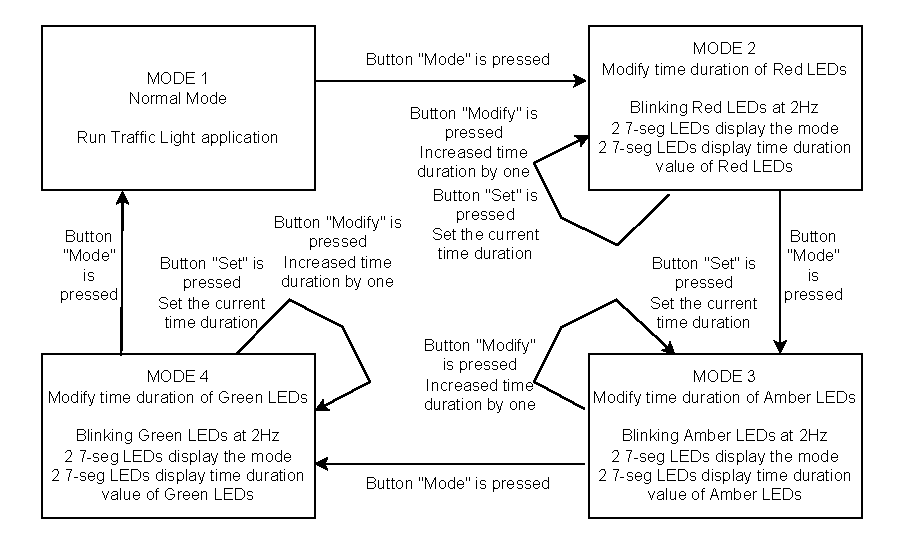
\includegraphics[width=0.95\linewidth]{Attachments/1.2.PDF}
\end{figure}
\subsubsection{Exercise 2: Proteus Schematic}
I used the 74HC595 IC to control the 4 seven-segment LEDs, replacing the LED scanning method from previous labs.
\label{ex2r1}
\begin{figure}[H]
	\centering
	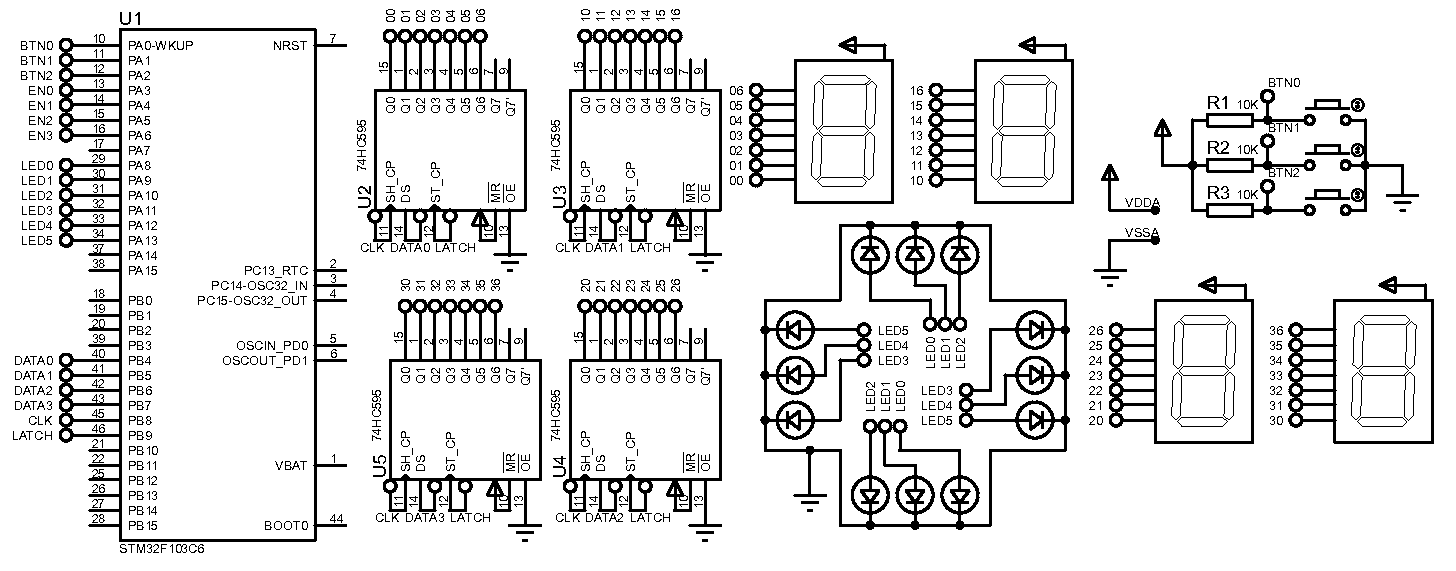
\includegraphics[width=0.95\linewidth]{Attachments/1.2.1.PDF}
\end{figure}
\newpage
\subsubsection{Exercise 3: Create STM32 Project}
\label{ex3r1}
\begin{figure}[H]
	\centering
	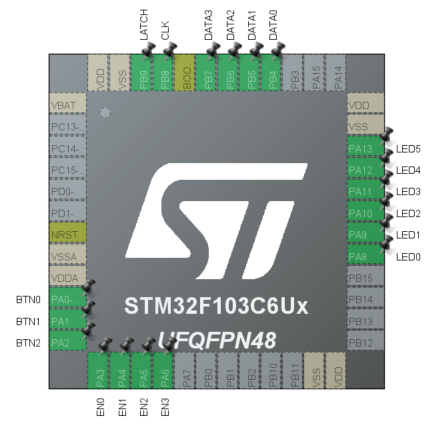
\includegraphics[width=0.95\linewidth]{Attachments/1.2.3.1.PNG}
\end{figure}
\label{ex3r2}
\begin{figure}[H]
	\centering
	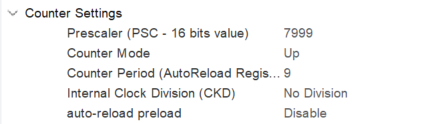
\includegraphics[width=0.95\linewidth]{Attachments/1.2.3.2.PNG}
\end{figure}
\newpage
\subsubsection{Exercise 4: Modify Timer Parameters}
\begin{itemize}
	\item[] To easily and efficiently modify the timer interrupt duration to 1 ms or 100 ms while keeping the system simple, we can retain the prescaler at 7999 and adjust the ARR (Counter Period) to 0 for 1 ms or 99 for 100 ms. In the code, we calculate the TIMER\_CYCLE based on the prescaler and ARR values and update the TIMER\_CYCLE variable in timer.c accordingly to maintain the 2 Hz LED blinking frequency and other system functionalities.
	\item[] Updating TIMER\_CYCLE: In timer.c, the TIMER\_CYCLE variable is set to 1 (for 1 ms interrupts) or 100 (for 100 ms interrupts) to ensure the soft timer logic correctly scales the duration (e.g., 500 ms for 2 Hz LED blinking) without affecting the system's overall behavior, such as the LED blinking frequency.
	\item[] This approach minimizes changes to the system by keeping the prescaler constant and only modifying the ARR and TIMER\_CYCLE, ensuring simplicity and compatibility with the traffic light application's requirements.
\end{itemize}
\begin{lstlisting}
# * timer.c	

#include "main.h"
#include "input_reading.h"

#define MAX_SOFT_TIMER 3

int TIMER_CYCLE = 10;

int timer_counter[MAX_SOFT_TIMER];
int timer_flag[MAX_SOFT_TIMER];

void setSoftTimer(int index, int duration) {
	if (index < MAX_SOFT_TIMER) {
		timer_counter[index] = duration / TIMER_CYCLE;
		timer_flag[index] = 0;
	}
}

void softTimer_run() {
	for (int i = 0; i < MAX_SOFT_TIMER; i++) {
		if (timer_counter[i] > 0) {
			timer_counter[i]--;
			if (timer_counter[i] == 0) timer_flag[i] = 1;
		}
	}
}

void HAL_TIM_PeriodElapsedCallback ( TIM_HandleTypeDef * htim )
{
	if(htim -> Instance == TIM2 ){
		softTimer_run();
		button_reading();
	}
}
\end{lstlisting}
\newpage
\subsubsection{Exercise 5: Adding code for button debouncing}
\begin{itemize}
	\item[] \textbf{Button debouncing}
	\begin{itemize}
		\item[] Two buffers (debounceButtonBuffer1 and debounceButtonBuffer2) store consecutive readings of each button.
		\item[] At every sampling cycle (for example, every 10ms), the program reads the button state again:
		\begin{itemize}
			\item[] If the two consecutive readings are the same, the signal is considered stable, and the confirmed state is stored in buttonBuffer.
			\item[] If the readings are different, it means the button is bouncing, so the program ignores the change.
		\end{itemize}
		\item[] This way, only a stable press or release is accepted as a valid input, effectively filtering out noise and mechanical bouncing.
	\end{itemize}
\end{itemize}
\begin{lstlisting}
# * input_reading.c	
	
#include "main.h"

#define N0_OF_BUTTONS 3

#define DURATION_FOR_AUTO_INCREASING 100

#define BUTTON_IS_PRESSED GPIO_PIN_RESET
#define BUTTON_IS_RELEASED GPIO_PIN_SET

static GPIO_PinState buttonBuffer [N0_OF_BUTTONS];

static GPIO_PinState debounceButtonBuffer1[N0_OF_BUTTONS];
static GPIO_PinState debounceButtonBuffer2[N0_OF_BUTTONS];

static uint8_t flagForButtonPress1s [ N0_OF_BUTTONS ];
static uint8_t flagForButtonPressedOnce[N0_OF_BUTTONS];

static uint16_t counterForButtonPress1s [ N0_OF_BUTTONS ];

GPIO_TypeDef* buttonPort[N0_OF_BUTTONS] = {BTN0_GPIO_Port, BTN1_GPIO_Port, BTN2_GPIO_Port};
uint16_t buttonPin[N0_OF_BUTTONS] = {BTN0_Pin, BTN1_Pin, BTN2_Pin};

void button_reading ( void ){
	for ( int i = 0; i < N0_OF_BUTTONS ; i ++){
		debounceButtonBuffer2 [i] = debounceButtonBuffer1 [i];
		debounceButtonBuffer1 [i] = HAL_GPIO_ReadPin ( buttonPort[i] , buttonPin[i] );
		if( debounceButtonBuffer1 [i] == debounceButtonBuffer2 [i]){
			if (buttonBuffer[i] == BUTTON_IS_RELEASED && debounceButtonBuffer1[i] == BUTTON_IS_PRESSED) flagForButtonPressedOnce[i] = 1;
			else flagForButtonPressedOnce[i] = 0;
			buttonBuffer [i] = debounceButtonBuffer1 [i];
		}
		if( buttonBuffer [i] == BUTTON_IS_PRESSED ){
			if( counterForButtonPress1s [i] < DURATION_FOR_AUTO_INCREASING ) counterForButtonPress1s [i ]++;
			else flagForButtonPress1s [i] = 1;
		} else {
			flagForButtonPressedOnce[i] = 0;
			counterForButtonPress1s [i] = 0;
			flagForButtonPress1s [i] = 0;
		}
	}
}

unsigned char is_button_pressed ( uint8_t index ){
	if( index >= N0_OF_BUTTONS ) return 0;
	return ( buttonBuffer [ index ] == BUTTON_IS_PRESSED );
}

unsigned char is_button_pressed_once(uint8_t index) {
	if(index >= N0_OF_BUTTONS) return 0;
	if(flagForButtonPressedOnce[index] == 1) {
		flagForButtonPressedOnce[index] = 0;
		return (flagForButtonPressedOnce[index] == 0);
	}
	return (flagForButtonPressedOnce[index] == 1);
}

unsigned char is_button_pressed_1s ( uint8_t index ){
	if( index >= N0_OF_BUTTONS ) return 0;
	return ( flagForButtonPress1s [ index ] == 1);
}
\end{lstlisting}
\begin{itemize}
	\item[] \textbf{Mode Switching}
	\begin{itemize}
		\item[] Each time the button is pressed once (is\_button\_pressed\_once(0)), the value of mode increases by 1.
		\item[] When mode exceeds 4, it returns to 1, allowing the user to cycle through four modes in sequence.
		\item[] There are two switch(mode) structures in the code, and each has a different purpose:
		\begin{itemize}
			\item[] \textbf{Initialization switch}
			\item[] It updates last\_mode and calls an initialization function corresponding to the selected mode.
			\item[] These functions are used to reset variables, timers, or LEDs so the new mode starts in a defined state.
			\item[] \textbf{Continuous execution switch}
			\item[] This part executes repeatedly inside the main while(1) loop while the mode remains the same.
			\item[] It calls the finite state machine (FSM) function for the current mode, allowing the system to continuously perform its tasks — for example, controlling the traffic lights or updating the modification timing logic.
		\end{itemize}
	\end{itemize}
\end{itemize}
\begin{lstlisting}
# * part of main.c
	
int last_mode = 1;
int mode = 1;

while (1)
{
	fsm_for_input_processing();
	fsm_for_led_display();
	
	if(is_button_pressed_once(0)) mode++;
	if(mode > 4) mode = 1;
	
	if (mode != last_mode) {
		last_mode = mode;
		switch(mode) {
			case 1: traffic_Init(); break;
			case 2: modifySec_Init(0); break;
			case 3: modifySec_Init(1); break;
			case 4: modifySec_Init(2); break;
		}
	}
	else {
		switch(mode){
			case 1: fsm_for_trafic_light(); break;
			case 2: fsm_for_traffic_modifySec(0); break;
			case 3: fsm_for_traffic_modifySec(1); break;
			case 4: fsm_for_traffic_modifySec(2); break;
		}
	}
}
\end{lstlisting}
\newpage
\subsubsection{Exercise 6: Adding code for displaying modes}
\begin{itemize}
	\item[] \textbf{Display mode on seven-segment LEDs}
	\begin{itemize}
		\item[] The function update7SEG() controls four seven-segment displays using a shift register mechanism.
		\item[] Each segment pattern is defined in the segmentMap[] array, where each bit represents one segment of a digit (from 0 to 9).
		\begin{itemize}
			\item[] The current values to be shown on the displays are stored in the seg\_buffer[4] array.
			\item[] During each update cycle, update7SEG() shifts out the bit patterns of all four digits (using DATAx and CLK pins), and finally sends a latch pulse (LATCH pin) to update the output of the shift registers.
		\end{itemize}
		\item[] By modifying the values in seg\_buffer[], the program can display numbers or mode indicators on the seven-segment LEDs.
	\end{itemize}
	\item[] \textbf{Blinking LEDs depending on the mode that is selected}
	\begin{itemize}
		\item[] The array led\_buffer[6] stores the ON/OFF states of six indicator LEDs.
		\item[] The function updateLED() writes these states to the physical GPIO pins connected to each LED.
		\item[] The finite state machine function fsm\_for\_led\_display() is called continuously in the main loop.
		\item[] A software timer (timer\_flag[0]) is used to trigger periodic updates — every 100ms.
		\item[] The timer ensures that LED updates happen at regular intervals, producing a stable and visible blinking effect.
	\end{itemize}
\end{itemize}
\begin{lstlisting}
# * led_display.c

#include "main.h"
#include "timer.h"

#define SEG_HIGH GPIO_PIN_RESET
#define SEG_LOW  GPIO_PIN_SET
#define LED_HIGH GPIO_PIN_SET
#define LED_LOW  GPIO_PIN_RESET

uint8_t segmentMap[11] = {
	0b0000001, 0b1001111,
	0b0010010, 0b0000110,
	0b1001100, 0b0100100,
	0b0100000, 0b0001111,
	0b0000000, 0b0000100,
	0b1111111
};

uint16_t ENPin[4] = {
	EN0_Pin, EN1_Pin,
	EN2_Pin, EN3_Pin
};

GPIO_TypeDef* ENPort[4] = {
	EN0_GPIO_Port, EN1_GPIO_Port,
	EN2_GPIO_Port, EN3_GPIO_Port
};

uint16_t LEDPin[6] = {
	LED0_Pin, LED1_Pin,
	LED2_Pin, LED3_Pin,
	LED4_Pin, LED5_Pin
};

GPIO_TypeDef* LEDPort[6] = {
	LED0_GPIO_Port, LED1_GPIO_Port,
	LED2_GPIO_Port, LED3_GPIO_Port,
	LED4_GPIO_Port, LED5_GPIO_Port
};

int led_buffer[6] = {0, 0, 0, 0, 0, 0};
int seg_buffer[4] = {0, 0, 0, 0};

void updateLED(){
	for(int i = 0; i < 6; i++) HAL_GPIO_WritePin(LEDPort[i], LEDPin[i], led_buffer[i] ? LED_HIGH : LED_LOW);
}

void update7SEG() {
	for (int i = 7; i >= 0; i--) {
		HAL_GPIO_WritePin(DATA0_GPIO_Port, DATA0_Pin, (segmentMap[seg_buffer[0]] >> i) & 1);
		HAL_GPIO_WritePin(DATA1_GPIO_Port, DATA1_Pin, (segmentMap[seg_buffer[1]] >> i) & 1);
		HAL_GPIO_WritePin(DATA2_GPIO_Port, DATA2_Pin, (segmentMap[seg_buffer[2]] >> i) & 1);
		HAL_GPIO_WritePin(DATA3_GPIO_Port, DATA3_Pin, (segmentMap[seg_buffer[3]] >> i) & 1);
		
		HAL_GPIO_WritePin(CLK_GPIO_Port, CLK_Pin, GPIO_PIN_SET);
		HAL_Delay(1);
		HAL_GPIO_WritePin(CLK_GPIO_Port, CLK_Pin, GPIO_PIN_RESET);
	}
	
	HAL_GPIO_WritePin(LATCH_GPIO_Port, LATCH_Pin, GPIO_PIN_SET);
	HAL_Delay(1);
	HAL_GPIO_WritePin(LATCH_GPIO_Port, LATCH_Pin, GPIO_PIN_RESET);
}

void resetBuffer(void){
	for(int i = 0; i < 6; i++) led_buffer[i] = 0;
	for(int i = 0; i < 4; i++) seg_buffer[i] = 0;
	updateLED();
	update7SEG();
}

void led_display_Init(){
	setSoftTimer(0, TIMER_CYCLE);
}

void fsm_for_led_display()
{
	if (timer_flag[0] == 1) {
		timer_flag[0] = 0;
		setSoftTimer(0, 100);
		
		updateLED();
		update7SEG();
	}
}
\end{lstlisting}
\newpage
\subsubsection{Exercise 7-8-9: Adding code for increasing time duration value for the
	red LEDs, amber LEDs and green LEDs}
\begin{itemize}
	\item[] \textbf{second button to increase the time duration value}
	\item[] The second button (is\_button\_pressed\_once(1)) is used to increase the current time value (tempSec) of the selected light.
	\item[] Each press increases the temporary time by one second, and this value is shown on the 7-segment display.
	\item[] \textbf{third button to set the value}
	\item[] The third button (is\_button\_pressed\_once(2)) is used to confirm and save the new duration value.
	\item[] When pressed, it updates the corresponding variable (redSec, yellowSec, or greenSec) using trafficSecCompute().
	\item[] The new values are then applied to the normal traffic mode the next time it runs.
\end{itemize}
\begin{lstlisting}
# * traffic_light.c

#include "main.h"
#include "timer.h"
#include "led_display.h"

typedef enum {
	STATE_RED_GREEN = 0,
	STATE_RED_YELLOW = 1,
	STATE_GREEN_RED = 2,
	STATE_YELLOW_RED = 3
} TrafficState;

TrafficState trafficState;

int redSec = 5;
int yellowSec = 2;
int greenSec = 3;

int countdownSec = 0;
int countdownSec7Seg[2] = {0 ,0};

int blinkState = 0;
int tempSec = 0;
int lastPressState0 = 0;
int pressState0 = 0;
int lastPressState1 = 0;
int pressState1 = 0;

void trafficSetLED(){
	for (int i = 0; i < 6; i++) led_buffer[i] = 0;
	switch (trafficState) {
		case STATE_RED_GREEN:
		led_buffer[0] = 1;
		led_buffer[5] = 1;
		break;
		case STATE_RED_YELLOW:
		led_buffer[0] = 1;
		led_buffer[4] = 1;
		break;
		case STATE_GREEN_RED:
		led_buffer[2] = 1;
		led_buffer[3] = 1;
		break;
		case STATE_YELLOW_RED:
		led_buffer[1] = 1;
		led_buffer[3] = 1;
		break;
	}
}

void trafficSet7Seg(){
	int a = countdownSec7Seg[0];
	int b = countdownSec7Seg[1];
	
	if (a < 0) a = 0;
	if (a > 99) a = 99;
	seg_buffer[0] = (a / 10) % 10;
	seg_buffer[1] = a % 10;
	
	if (b < 0) b = 0;
	if (b > 99) b = 99;
	seg_buffer[2] = (b / 10) % 10;
	seg_buffer[3] = b % 10;
}

void trafficSecCompute(int redsec, int yellowsec, int greensec){
	if(redsec != 0){
		redSec = redsec;
		greenSec = redsec - yellowSec;
	}
	if(yellowsec != 0){
		yellowSec = yellowsec;
		greenSec = redSec - yellowsec;
	}
	if(greensec != 0){
		greenSec = greensec;
		redSec = greensec + yellowSec;
	}
}

void traffic_Init(){
	resetBuffer();
	trafficState = STATE_RED_GREEN;
	trafficSecCompute(0, 0, 0);
	countdownSec = greenSec;
	countdownSec7Seg[0] = redSec;
	countdownSec7Seg[1] = greenSec;
	setSoftTimer(1, TIMER_CYCLE);
}

void modifySec_Init(int whichsec){
	resetBuffer();
	setSoftTimer(2, TIMER_CYCLE);
	tempSec = whichsec == 0 ? redSec : (whichsec == 1 ? yellowSec : greenSec);
}

void fsm_for_trafic_light(){
	if (timer_flag[1]) {
		timer_flag[1] = 0;
		setSoftTimer(1, 1000);
		
		trafficSecCompute(0, 0, 0);
		countdownSec7Seg[0]--;
		countdownSec7Seg[1]--;
		
		if (countdownSec == 0) {
			switch (trafficState) {
				case STATE_RED_GREEN:
				trafficState = STATE_RED_YELLOW;
				countdownSec7Seg[1] = yellowSec - 1;
				countdownSec = yellowSec;
				break;
				case STATE_RED_YELLOW:
				trafficState = STATE_GREEN_RED;
				countdownSec7Seg[0] = greenSec - 1;
				countdownSec7Seg[1] = redSec - 1;
				countdownSec = greenSec;
				break;
				case STATE_GREEN_RED:
				trafficState = STATE_YELLOW_RED;
				countdownSec7Seg[0] = yellowSec - 1;
				countdownSec = yellowSec;
				break;
				case STATE_YELLOW_RED:
				trafficState = STATE_RED_GREEN;
				countdownSec7Seg[0] = redSec - 1;
				countdownSec7Seg[1] = greenSec - 1;
				countdownSec = greenSec;
				break;
			}
		}
		
		countdownSec--;
		if (countdownSec < 0) countdownSec = 0;
		
		trafficSetLED();
		trafficSet7Seg();
	}
}

void fsm_for_traffic_modifySec(int whichsec){
	if (timer_flag[2]) {
		timer_flag[2] = 0;
		setSoftTimer(2, 250);
		
		blinkState = !blinkState;
		for(int i = 0; i < 6; i++) led_buffer[i] = (i == whichsec || i == whichsec + 3) ? blinkState : 0;
	}
	
	seg_buffer[0] = 0;
	seg_buffer[1] = whichsec + 2;
	seg_buffer[2] = (tempSec / 10) % 10;
	seg_buffer[3] = tempSec % 10;
	
	if(is_button_pressed_once(1)) pressState0 = !pressState0;
	if (pressState0 != lastPressState0) {
		lastPressState0 = pressState0;
		
		tempSec++;
	}
	
	if(is_button_pressed_once(2)) pressState1 = !pressState1;
	if (pressState1 != lastPressState1) {
		lastPressState1 = pressState1;
		
		switch(whichsec) {
			case 0: trafficSecCompute(tempSec, 0, 0); break;
			case 1: trafficSecCompute(0, tempSec, 0); break;
			case 2: trafficSecCompute(0, 0, tempSec); break;
		}
		tempSec = whichsec == 0 ? redSec : (whichsec == 1 ? yellowSec : greenSec);
	}
}
\end{lstlisting}
\subsubsection{Exercise 10: To finish the project}
The Youtube link for my demo:
\textcolor{blue}{\url{https://hehehaha.com}}
\end{document}


